\chapter{Pin-Injection Automation für Diehl Aviation}
\label{ch:pia}

Das zu programmierende Projekt \ac{pia} wird für den Kunden Diehl Aviation
\footnote{\url{https://www.diehl.com/aviation/de/}} entwickelt, welches als semi-
automatisiertes Pin Injection Testing Programm fungieren soll.

Der Kunde Diehl muss die von ihnen entwickelten Geräte auf viele bestimmte Eigenschaften und
Ereignisse \ac{bzw} auch auf Gefahren testen, welche während eines Fluges auftreten können.
Einer dieser Tests ist der sogenannte Pin-Injection Test.
Bei diesem Test werden die Pins eines Fluggerätes auf Störungen und auch Beschädigungen im
Rahmen der Umweltqualitätsprüfung nach \cite{DO-160} getestet. Jeder Pin besitzt ein Interface
zum steuern von verschiedenen im Gerät verbauten Schaltern. Da jedes Interface andere
Eigenschaften besitzt, hat dementsprechend jedes dieser Interfaces unterschiedliche
Anforderungen (engl: "Requirements") die getestet werden müssen.
Demzufolge ist das Testen der Pins \ac{bzw} der Geräte sehr zeitaufwändig und kann im
Durchschnitt bis zu zwei Wochen dauern, je nachdem wie viele Pins das zu testende Gerät
besitzt.

\ac{pia} soll die Tests, welche normalerweise von einem Mitarbeiter von Hand abgearbeitet
werden, einlesen und nur durch eine vom Mitarbeiter angefertigte Konfigurationsdatei
automatisieren und verarbeiten.

\pagebreak
Abbildung \ref{fig:flight_unit} zeigt den Aufgebauten Test an einer Flight Unit\footnote{\url{https://www.diehl.com/aviation/de/portfolio/avionics/}}, welcher noch von Hand abgearbeitet wurde.

\begin{figure}[H]
	\centering
	\includegraphics[width=0.8\textwidth, height=0.6\textwidth]{graphics/PinInjectionTest_FlightUnit.png}
	\caption{Pin-Injection Test Flight Unit}
	\label{fig:flight_unit}
\end{figure}


\section{Projekteinarbeitung}
\label{sec:prj-einarbeitung}

Da das Projekt erst kurz vor meinem ersten Arbeitstag angenommen und mit Diehl beschlossen
wurde, stand bis auf die Aufgabenanforderung der Software noch nichts fest. Dementsprechend
konnte ich später in vielen Bereichen wie \ac{zb} die Programmiersprache oder auch die
Programmstruktur frei wählen und auch viele meiner Ideen mit ins Programm einfließen lassen.
Meine erste Aufgabe war es erst einmal das Verständnis für den eigentlichen Test zu bekommen,
welcher das Programm automatisieren soll, denn zu diesem Zeitpunkt war der vom Programm
ab zulaufende Testzyklus noch nicht vollständig festgelegt. 


\subsection{Aufgabe der zu programmierenden Software}
\label{subsec:aufgabe-software}

Die Aufgabe der zu entwickelten Software besteht darin, dass eine vom Mitarbeiter erstellte
Testkonfigurationsdatei, welche normalerweise von Hand abgearbeitet wird, eingelesen und
verarbeitet wird. Am Ende soll eine sogenannte Result Ouput Log File die Ausgaben der
Programmauswertung abspeichern und angeben ob ein Test gescheitert ist oder alles normal
verlief.
Bei der Verarbeitung eines Test Schritts wird ein Roboter angesteuert der maximal zwei
sogenannte Bananenstecker auf ein Board steckt, welches mit den Pins des zu testenden Gerätes
angeschlossen ist. Danach kann ein optionales \ac{micbac} Kommando an das am Pin anliegende
Interface geschickt werden, welches \ac{zb} einen internen Schalter umlegt. Danach wird ein
Puls mehrmals auf den Pin gefeuert. Dieser Puls hat eine vorgegebene Wellenform (engl:
"Waveform"), welche von einem angeschlossen Puls Generator generiert wird. Der Puls Generator
ist zugleich auch für die Anzahl der zu feuernden Pulse zuständig. Nach dem letzten
abgefeuerten Puls wird ein Bild vom Oszilloskop abgespeichert und mit einem vorher
aufgenommenen Referenzbild verglichen, um zu schauen ob der Pin \ac{bzw} sogar das komplette
Gerät beschädigt wurde oder ob alles in normal verlaufenden Bereich liegt. 


\subsection{Entwicklung der Programmstruktur}
\label{subsec:entw-prgstr}

Während meiner Praxisphase war die Entwicklung und im späteren Verlauf auch die
Weiterentwicklung der Programmstruktur ein großer Bestandteil meiner Arbeit. Da die Entwicklung
zum Teil etappenweise voran ging, mussten Teile der Programmstruktur relativ schnell und ohne
wirklich großen Aufwand modifizierbar, erweiterbar und zu einem gewissen Teil auch austauschbar
sein. 

\begin{figure}[H]
	\centering
	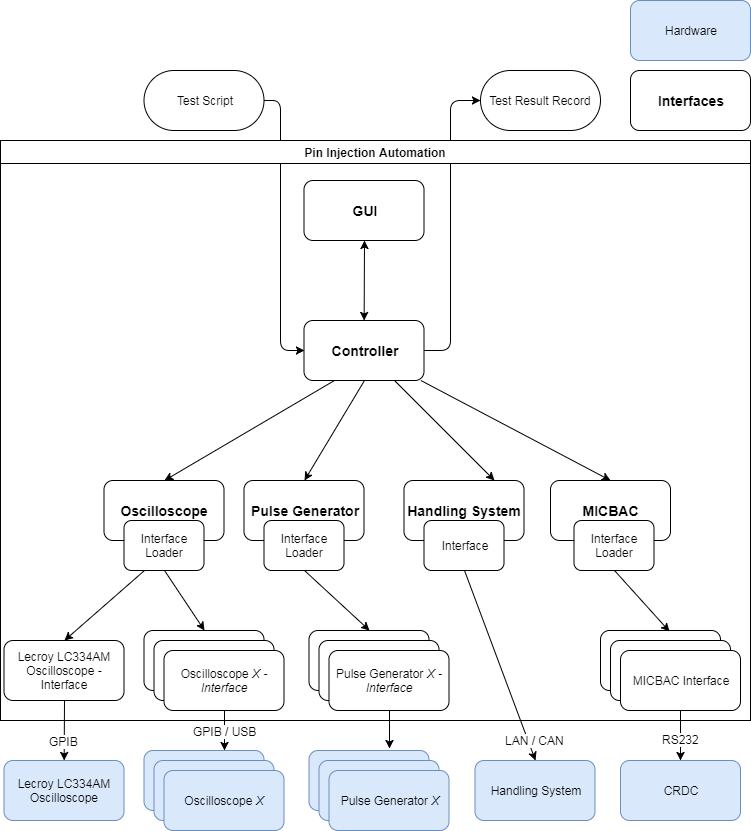
\includegraphics[width=0.75\textwidth, height=0.75\textwidth]{graphics/program_architecture.png}
	\caption{Programm Architektur}
	\label{fig:prg_architecture}
\end{figure}

Abbildung \ref{fig:prg_architecture} zeigt die entwickelte abstrakte Programmstruktur,
welche im Programm auch umgesetzt und benutzt wurde. Dort sieht man auch, dass das Programm
mehrere Interfaces für Oszilloskope und Puls-Generatoren ansteuert. Diese Anforderung wurde am
Ende so implementiert, dass sofern irgendeine neue Hardware Komponente eingebettet werden soll,
nur kleine Teile wie \ac{zb} die Auswahlmöglichkeit in der \ac{gui} erweitert werden muss. Die
eigentliche Programmstruktur wird dadurch nicht verändert, was die Flexibilität erhöht und es
so möglich ist das Programm nur durch hinzufügen einer neuen Datei, unter der Einhaltung von
einer bestimmten  Namensvergebung, zu erweitern. Erkennbar ist auch, dass die Aufgaben in
unterschiedliche Interfaces unterteilt wurden, was die Programmübersicht erhöht und  interne
Abhängigkeiten verringert. Dadurch sind \ac{zb} teile der \ac{gui} des öfteren ohne großen
aufwand schnell austauschbar gewesen, was mir im Verlaufe des Praktikums öfters mal sehr viel
Zeit eingespart hat.

	
\subsection{Python 3 als Programmiersprache}
\label{subsec:py3_as_lang}

Wie schon in Kapitel \ref{sec:prj-einarbeitung} erwähnt war es mir frei zu wählen, in welcher
Programmiersprache ich das Projekt realisieren möchte. Meine Entscheidung fiel dabei schnell
auf \cite{Python} 3, da auch die Erfahrung mit dieser Sprache auf der Seite des Kunden sehr 
groß war. Den Vorteil in dieser Sprache sehe ich darin, dass \cite{Python} eine sehr aktuelle 
und dynamische Programmiersprache ist, welche sich schnell weiterentwickelt. 

Das Hauptmerkmal von \cite{Python} ist die Lesbarkeit und wird durch Code Style Richtlinien und
Idiome realisiert. Diese Lesbarkeit wird auch \textit{Pythonic Way} genannt. Die Idiome in
\cite{Python} lassen zukünftige Leser genau verstehen, was der Code machen soll, während die
Code Style Richtlinien für einen einheitlichen Code sorgen.

Die Softwareanforderung wie \ac{zb} Datensätze aus einer \ac{csv} Datei auszulesen und zu 
verarbeiten konnte mit Hilfe der von \cite{Python} zur Verfügung gestellten \ac{api} sehr 
schnell realisiert werden. Des weiteren standen \cite{Python} Module für das Verarbeiten von 
\ac{micbac} Kommandos aus einem vorherigen Projekt bereits zur Verfügung.


\section{Die Erste Simulation}
\label{sec:first_simulation}

Die erste Aufgabe am Projekt war das erstellen einer Simulation. Die Simulation sollte am 
Anfang nur die Architektur implementieren und die Ausgabe für den Benutzer simulieren. Im 
Verlaufe des Praktikums wurden dann diese Ausgaben mit echten Werten verknüpft.

Um zu garantieren, dass die Softwarequalität bestehen bleibt, habe ich auf dem interen GitLab
\footnote{\url{https://about.gitlab.com/}} Server von Konzept einen sogenannten GitLab Runner
\footnote{\url{https://docs.gitlab.com/runner/}} erstellt. 


\subsection{Konfigurieren des GitLab Runner}
\label{subsec:gitlab_runner}

Um den Runner nicht jedes mal beim einchecken neu aufbauen zu müssen und die Daten immer mit 
den selben Eigenschaften eingecheckt werden, habe ich ein \cite{Docker} Image, ein 
Speicherabbild eines Containers, erstellt.

\cite{Docker} wird zur Isolierung von Anwendungen mit Containervirtualisierung genutzt. Diese 
Container gewährleisten die Trennung und Verwaltung der auf dem Rechner genutzten Ressourcen 
und vereinfacht die Bereitstellung von Anwendungen, weil sich die Container leicht als Dateien 
transportieren und installieren lassen.

\begin{figure}[H]
	\centering
	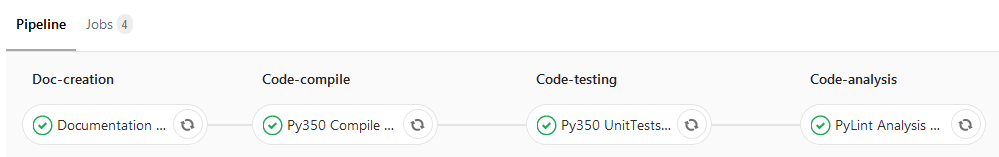
\includegraphics[width=1\textwidth, height=0.2\textwidth]{graphics/pipeline.png}
	\caption{Konfigurierte Pipeline}
	\label{fig:pipeline}
\end{figure}

In Abbildung \ref{fig:pipeline} stellt die Pipeline die Schritte dar, die durchlaufen werden.
Dazu gehört die Erstellung einer \ac{api} aus den Python Doc-Strings, die Code Kompilierung, 
das durchlaufen der Unit Tests und das durchlaufen von \cite{Pylint}. \cite{Pylint} ist ein 
statisches Codeanalyse Tool, das unter anderem den Code auf die Einhaltung der in \cite{PEP8} 
beschriebenen Regeln prüft.


\subsection{Einlesen von CSV-Dateien}
\label{subsec:read_csv}

Ein großer Bestandteil des Programms waren die eingelesenen Daten, welche in einem \ac{csv}-Dateiformat abgespeichert wurden. Diese Aufgabe habe ich mittels der Klasse \textit{DictReader} 
gelöst, welche in der \cite{Python} \ac{api} vorhanden ist. Diese Klasse liest jede Zeile der 
\ac{csv}-Datei in ein \textit{Dictionary} \ac{bzw} den Python Datentyp \textit{dict} ein. Ein 
\textit{Dictionary} ist eine unsortierte, veränderbare und indexierte Kollektion aus 
\textit{Key-Value-Paaren}. Die Klasse \textit{DictReader} nimmt die erste Zeile der \ac{csv}-
Datei als \textit{Keys} und fügt die restlichen Zeilen als \textit{Values} ein. 
Da der Reader beim einlesen von Daten sehr sensibel ist und bei einem falschen Format \ac{bzw} 
bei falschen \textit{Key}-Werten oder auch bei falschen \textit{Value}-Werten direkt Fehler 
wirft, mussten diese irgendwie abgefangen und behandelt werden. Ein Problem war das erkennen 
und überspringen von Kommentaren. Kommentare haben in einer Datei immer mit dem \textit{\#}-Zeichen angefangen. 
\pagebreak

\inputpython{scripts/read_csv.py}{1}{14}{Read From CSV-File}{lst:read_csv}

In dem Code Listing \ref{lst:read_csv} sieht man eine Zusammenfassung des Codes, welcher für 
das Einlesen der Daten zuständig ist und die Python-private Methode \textit{skip\_comments()}, 
welche Kommentare erkennen und überspringen soll. Die Kommentare sollten möglichst bevor die 
Daten als Wert in ein \textit{Dictionary} gespeichert werden herausgefiltert werden. Dies habe 
ich mit einem \ac{regex} (engl: Regular Expression) gelöst, welcher die Zeile nach dem 
\textit{\#}-Zeichen absucht und falls eins gefunden wurde alle nachgehenden Zeichen inklusive 
dem \textit{\#}-Zeichen in der Zeile subtrahiert und die subtrahiert Zeile dann wieder 
zurückgibt.


\subsection{Erstellung einer GUI}
\label{subsec:create_gui}

Nachdem die Textuelle Simulation abgeschlossen war machte ich mich an die Erstellung einer \ac{gui}. Da vom Projekt keine Vorgaben existierten, konnte ich bei vielen selbst Entscheiden wie diese implementiert werden.

\begin{figure}[H]
	\centering
	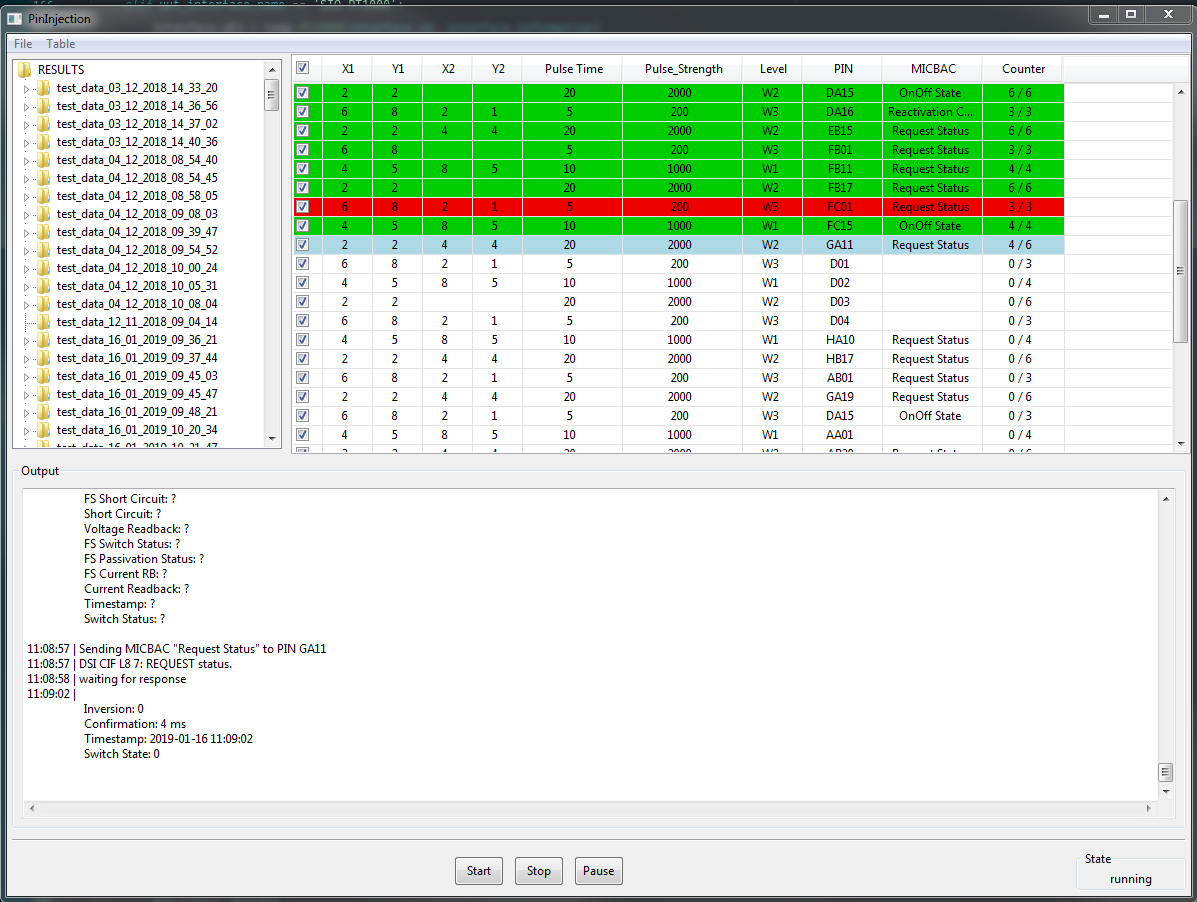
\includegraphics[width=1\textwidth, height=0.75\textwidth]{graphics/GUI.png}
	\caption{Graphical User Interface}
	\label{fig:pipeline}
\end{figure}

Die Grafik \ref{fig:pipeline} zeigt die \ac{gui}, wie sie am Ende des Praktikums implementiert wurde. Die Tablle, welche die Zeilen anzeigt, kann den gerade laufenden Test markieren, anzeigen ob die vorherigen Tests erfolgreich durchgelaufen sind oder nicht, einzelne Zeilen zum Testen auswählen und die Zeilen nach einer bestimmten Spalte sortieren. 
Die Tabelle wurde als virtuelle Tabelle implementiert. Das bedeutet, dass die Tabelle mit Hilfe der eingelesenen \ac{csv}-Datei indirekt adressiert wird und die Realisierung nicht direkt angesprochen wird. Damit war es sogar möglich eine \ac{csv}-Datei mit 1 Millionen Zeilen innerhalb von ca. 20-30 Sekunden einzulesen und anzuzeigen.